\documentclass[letter, 11pt]{article}
\usepackage{fullpage}
\usepackage[margin=0.5in]{geometry}
\usepackage{graphicx}
\usepackage{wrapfig}
\usepackage{caption}
\usepackage{subcaption}
\usepackage{listings}
\usepackage{hyperref}
\usepackage{amsmath}
\usepackage{float}

\pagenumbering{gobble}

\begin{document}
\noindent
\large \textbf{Rahul Ghosh} \hfill \textbf{Assignment\#4}\\
\normalsize Student ID: 5476965 \hfill CSci 5561\\


\section*{\centering CONVOLUTIONAL NEURAL NETWORK}

\subsection*{Methods}
\subsubsection*{Single-layer Linear Perceptron}
In this method each image is resized to a small fixed resolution to get a tiny image representation. The original image and the tiny image is compared in figure 1. This tiny image is transformed to a vector and normalized to get a zero mean and unit length vector. 

Finally KNN classification is used on the vectorized data. For \textbf{k = 10} the accuracy obtained is \textbf{23.8667} and the confusion matrix is shown in figure 2(a).

\subsubsection*{Single-layer Perceptron}
\subsubsection*{Multi-layer Perceptron}
\subsubsection*{Convolutional Neural Network}

\subsection*{Results}
\begin{figure}[H]
    \minipage{0.3\textwidth}
        \centering
        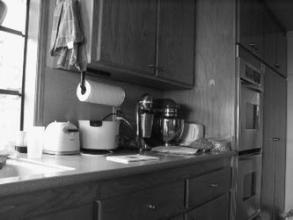
\includegraphics[width=\textwidth]{HW4/RESULT/original.png}
        \subcaption{Original Image}
    \endminipage\hfill
    \minipage{0.3\textwidth}
        \centering
        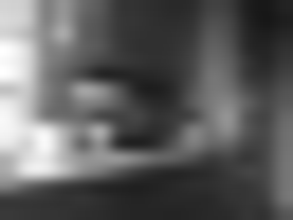
\includegraphics[width=\textwidth]{HW3/RESULT/tiny.png}
        \subcaption{Tiny Image}
    \endminipage\hfill
    \minipage{0.3\textwidth}
        \centering
        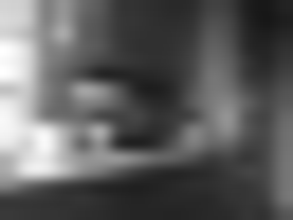
\includegraphics[width=\textwidth]{HW3/RESULT/tiny.png}
        \subcaption{Tiny Image}
    \endminipage\hfill
    \caption*{Figure 1}
\end{figure}

\begin{figure}[H]
    \minipage{0.33\textwidth}
        \centering
        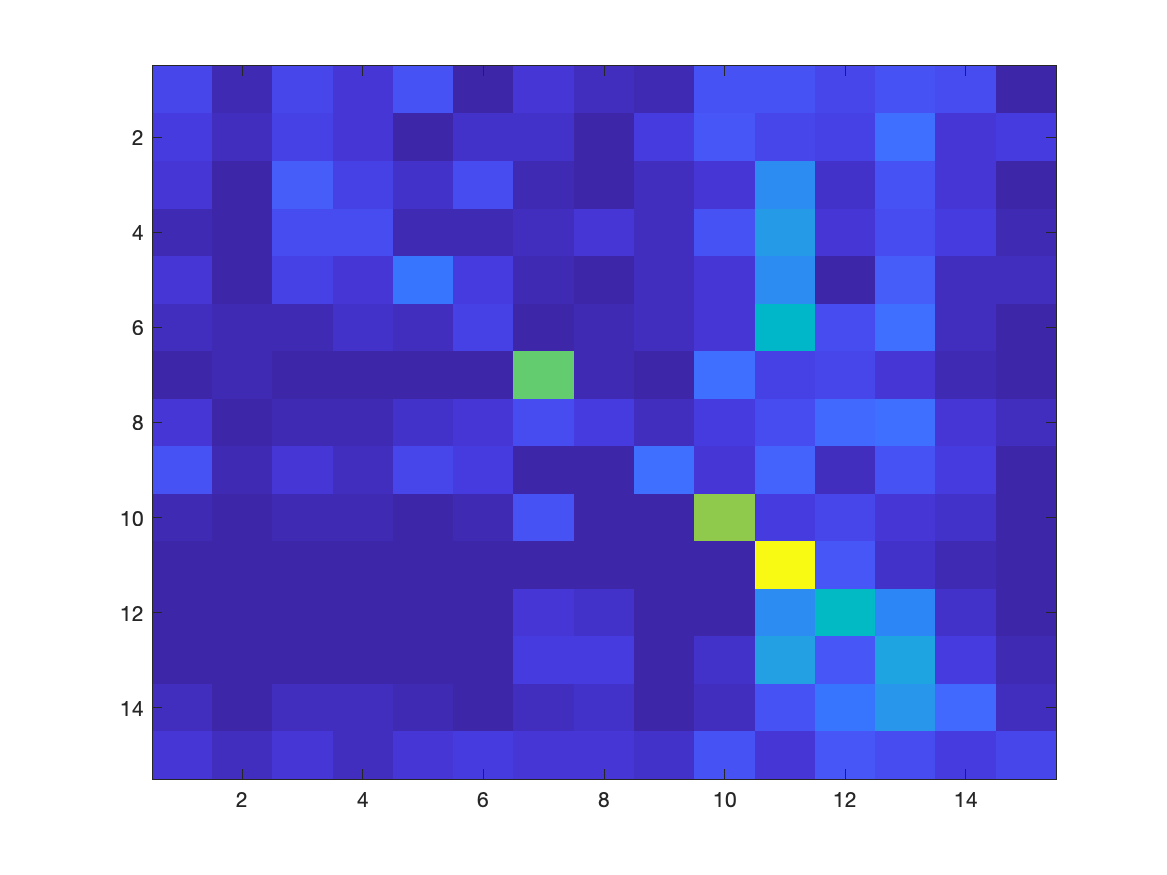
\includegraphics[width=\textwidth]{HW3/RESULT/ClassifyKNN_Tiny_confusion.png}
        \subcaption{Confusion matrix for Tiny-KNN}
    \endminipage\hfill
    \minipage{0.33\textwidth}
        \centering
        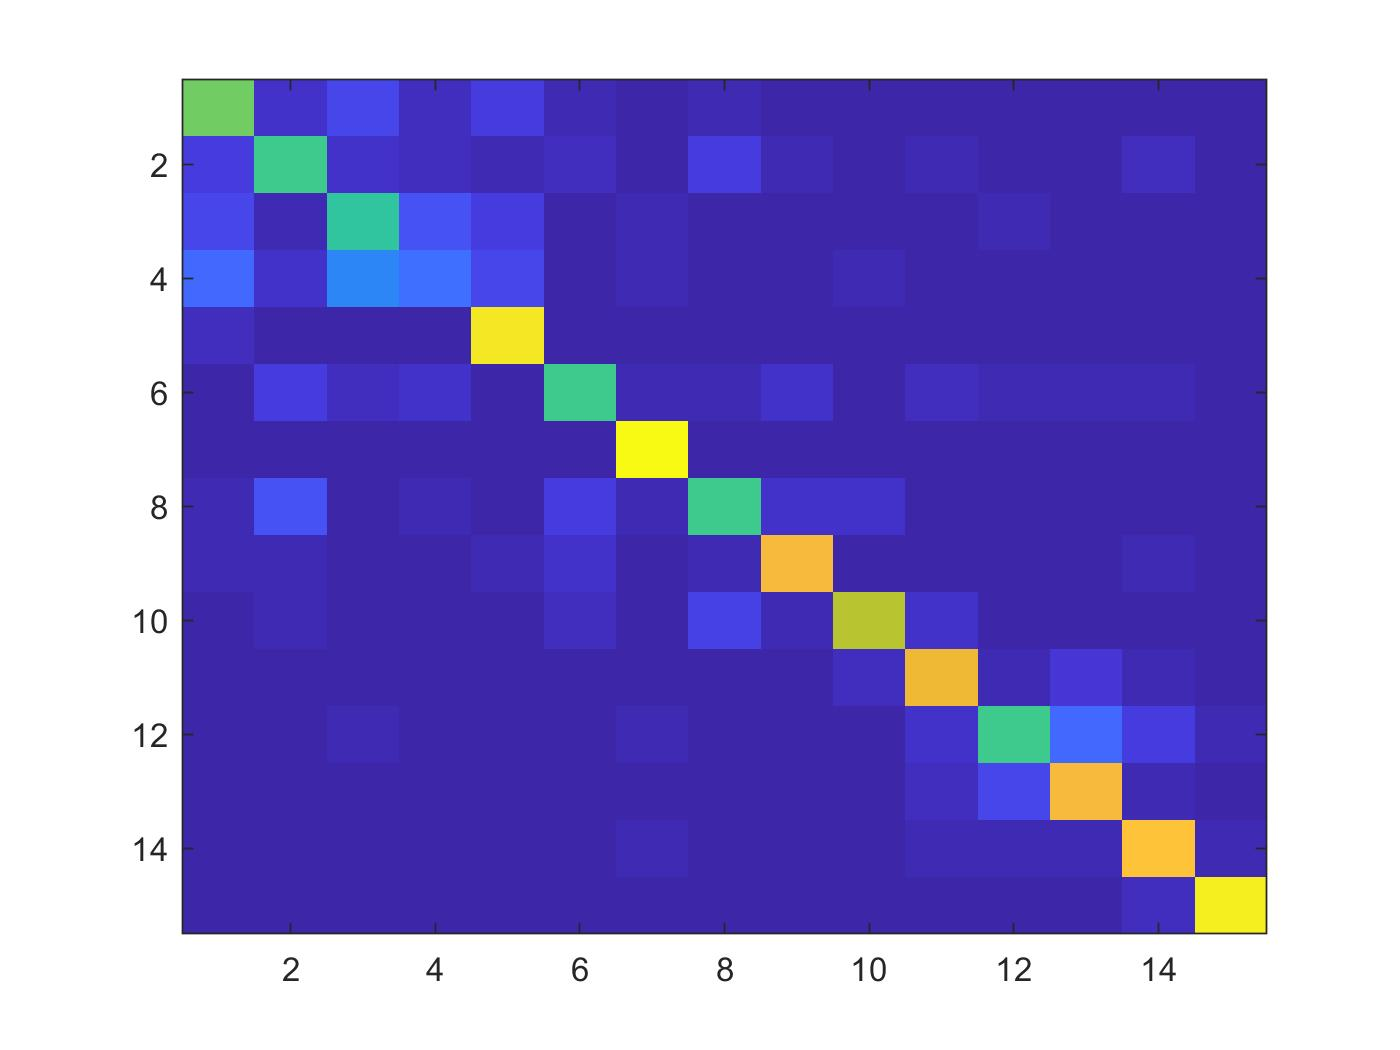
\includegraphics[width=\textwidth]{HW3/RESULT/ClassifyKNN_BOW_confusion.jpg}
        \subcaption{Confusion matrix for BoW+KNN}
    \endminipage\hfill
    \minipage{0.33\textwidth}
        \centering
        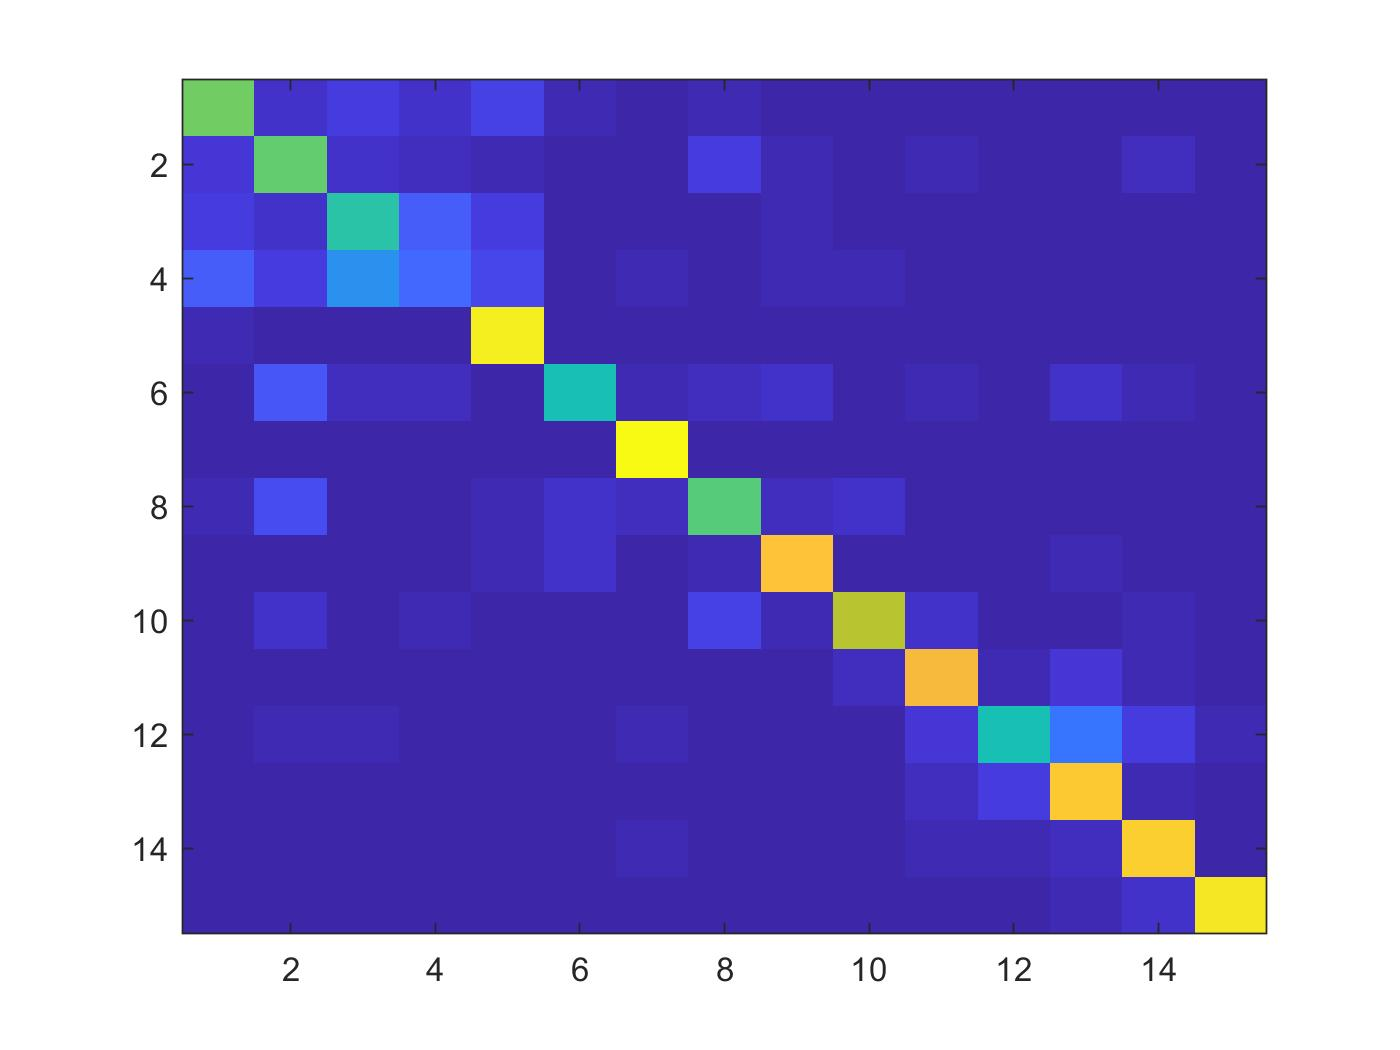
\includegraphics[width=\textwidth]{HW3/RESULT/ClassifySVM_BOW_confusion.jpg}
        \subcaption{Confusion matrix for BoW+SVM}
    \endminipage\hfill
    \caption*{Figure 2}
\end{figure}

\end{document}